\section{Component classes}

An important component of the installation in the house model is a thermal buffer vessel. The vessel is a storage for hot water which serves as a reservoir for thermal energy. When large enough, the vessel can mediate the heat demand of the house by allowing fast discharge and slow charge rates. Slow charge rates enable the use of heat pumps and electric heating with modest power ratings. The buffer vessel therefore plays a key role in replacing gas boilers, without the involvement of high-power flow-through heaters. 

In modelling a thermal buffer vessel, it is customary to discretize the vertical temperature gradient by imposing a \emph{stratified} geometry. In this way, a stable configuration is achieved, with warmer (water) layers on top of colder layers in the vessel. Thus, convection phenomena can be neglected, and interlayer thermal transport occurs by diffusion, driven by the thermal downward gradient.

\begin{figure}[H]
	\centering
	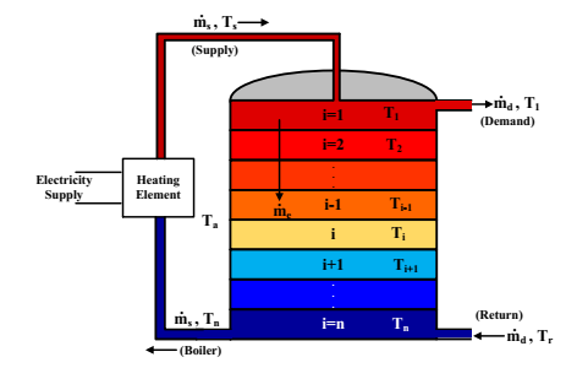
\includegraphics[width=0.5\columnwidth]{Pictures/stratified.png}
	\caption[Short title]{One-dimensional heat conduction in a stratified buffer vessel}
	\label{fig:stratified}
\end{figure} 

In the \textsf{housemodel/sourcesink} subpackage, a subpackage \textsf{buffervessels} is defined. The module buffer\_vessel.py contains a general class \textsf{StratifiedBuffer} with attributes and methods:

\lstinputlisting[label=lst:buffervessel, linerange={8-30}, 
caption={StratifiedBuffer class constructor}] 
{C:/Data/PROJECTS_NOVA/MCSE@BTO/FUTUREFACTORY/twozone_housemodel-git/housemodel/sourcesink/buffervessels/buffer_vessel.py}






















\newpage